\chapter{Bausteinsicht}
Die folgende Grafik zeigt den ersten Überblick über das System, welches in ihre Einzelheiten und ihre Micro Services zerlegt ist.
\begin{figure}[h]
	\centering
	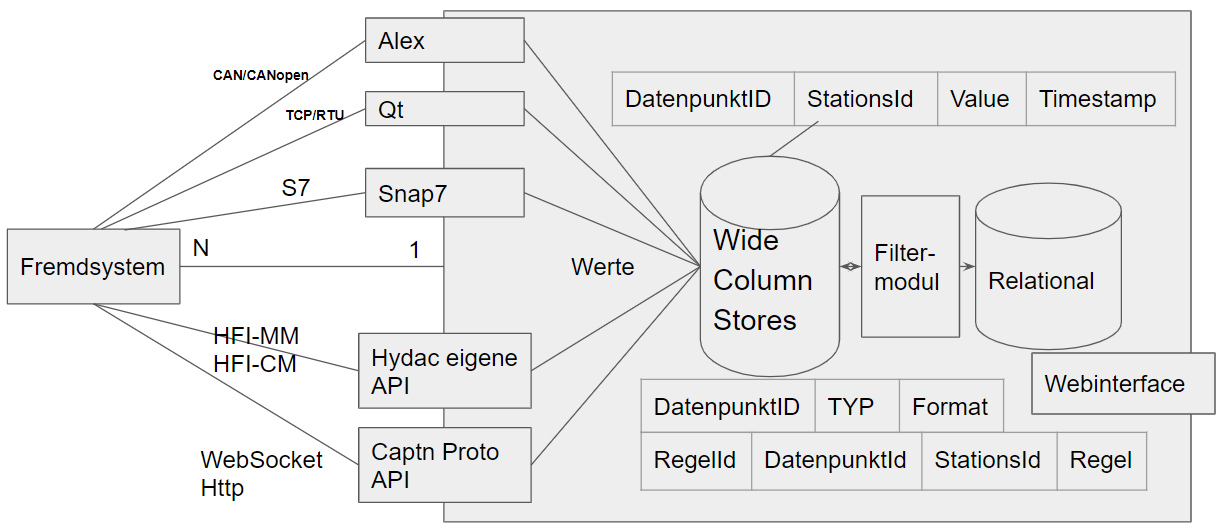
\includegraphics[width=1.0\textwidth]{Graphics/blackbox1.png}
	\caption{Erste Ebene}
	\label{fig:erste_ebene}
\end{figure}
Damit die die vielen Fremdsysteme und Maschinen mit unserer Software kommunizieren können, benötigen wir Implementierungen aller Protokolle in C++. Für CAN bzw. CANopen hat Alex eine Bibliothek in seiner Bachelorarbeit geschrieben. Für TCP/RTU nutzen wir Qt, für S7 gibt es Snap7. Die Hydac hat ihre eigene API und Bibliothek für die eigenen HFI-MM und HFI-CM Protokolle. Zu guter Letzt serialisieren wir WebSocket und HTTP mit Capn Proto. Alle Bibliotheken ermöglichen das einfache Abspeichern in den Wide-Column-Store oder bereiten es zumindest vor. Dafür werden eine DatenpunktID und StationsID der Maschine mit dem Wert und dem Zeitstempel gespeichert. Da diese Daten komplett ungeprüft in die Datenbank einfließen, muss ein weiterer Baustein alle Einträge überprüfen und Messfehler oder kritische Werte direkt in der Weboberfläche anzeigen. Dass die Überprüfung eventuell etwas langsamer als der Datenstrom in die Datenbank sein kann, ist an sich nicht schlimm, da die Anwendung in Produktionspausen aufholen und die noch ungeprüften Daten währenddessen verarbeitet.\\
In der relationalen Datenbank befinden sich dann die DatenpunktIDs mit ihren Typen und Formaten, damit man ein Schema zur Darstellung im Interface hat. zusätzlich zu den Nutzer- und Rechtedaten gibt es auch noch eine Tabelle, die Regeln für die Datenpunkte abbildet.\\
\begin{figure}[h]
	\centering
	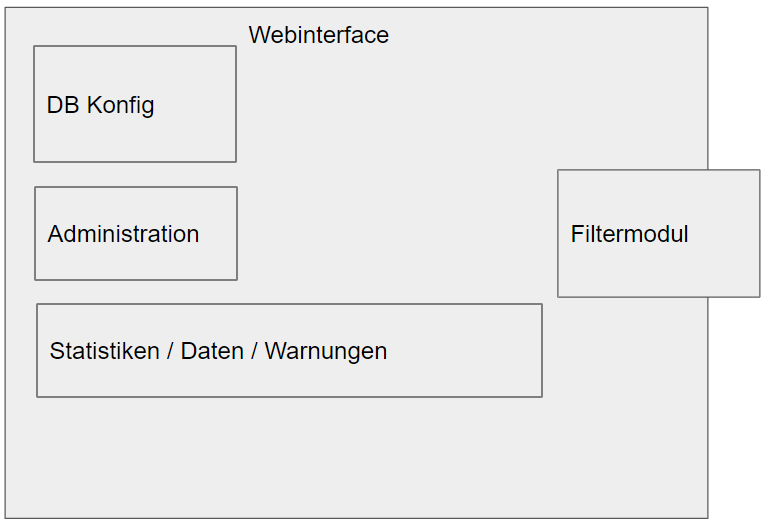
\includegraphics[width=0.7\textwidth]{Graphics/blackbox2.png}
	\caption{Zweite Ebene}
	\label{fig:zweite_ebene}
\end{figure}
Das Webinterface hat zu beiden Datenbanken eine Verbindung und kann auch die API des Filtermoduls mitbenutzen. In der Nutzeroberfläche wird zwischen einem administrativem und einem anwendungsspezifischen Teil unterschieden. In letzterem werden nur Daten und Statistiken aufbereitet angezeigt, während die Rechtevergabe und Feineinstellung in der Administratoroberfäche stattfindet. 